\chapter{项目设计方案}

\section{数据库设计}
在原有的饿了吧V1.0的数据库结构基础上,饿了吧V2.0对数据库进行了如下修改:
  \begin{enumerate}
      \item business表添加delTag字段
      \item food表添加delTag字段
      \item deliveryaddress表添加delTag字段
      \item delTag表示删除标记,其中0:正常,1:删除
      \item food表添加soudOut字段
      \item user .password成员的长度修改为70
      \item user表添加authorization成员,0:管理员,1:普通用户,2:商家用户
        \item user表添加businessId成员,无符号,添加外键,对business表businessId的引用
  \end{enumerate}
\subsection{DB一览表}
\begin{table}[h]
\resizebox{\columnwidth}{!}{%
\begin{tabular}{|l|l|l|l|}
\hline
\rowcolor[HTML]{FAFAFA} 
{\color[HTML]{262626} NO} & {\color[HTML]{262626} 表名称} & {\color[HTML]{262626} 中文名} & {\color[HTML]{262626} 说明} \\ \hline
1 & business        & 商家表    & 存储所有商家信息          \\ \hline
2 & food            & 食品表    & 存储每个商家拥有得食品得的所有信息 \\ \hline
3 & cart            & 购物车表   & 存储每个用户的购物车中的食品信息  \\ \hline
4 & deliveryaddress & 送货地址表  & 存储每个用户的所有送货地址信息   \\ \hline
5 & orders          & 订单表    & 存储每个用户的所有订单信息     \\ \hline
6 & orderdetailet   & 订单明细吧表 & 存储每个订单中的所有食品信息    \\ \hline
7 & user            & 用户表    & 存储所有用户的信息         \\ \hline
\end{tabular}%
}
\caption{数据库一览表}
\label{tab:dbyl}
\end{table}

\subsection{表结构}
约束类型标识: PK:primary key 主键 FK:foreign key 外键 NN:not null 非空 UQ:unique 唯一索引 AI:auto increment 自增长列  \par
删除标记:数据类型int,正常:0    删除:1\par
点餐分类: 1:美食、2: 早餐、3:跑腿代购、4:汉堡 披萨、5:甜品饮品、6:速食 简餐、7:地方小吃、8:米粉 面馆、9:包子粥铺、10:炸 鸡炸串
\subsubsection{business(商家表)}
\begin{table}[H]
\resizebox{\columnwidth}{!}{%
\begin{tabular}{|l|l|l|l|l|l|l|}
\hline
NO & 字段名             & 数据类型       & size  & 默认值  & 约束       & 说明   \\ \hline
1  & businessId      & int        &       &      & PK AI NN & 商家编号 \\ \hline
2  & businessName    & varchar    & 40    &      & NN       & 商家名称 \\ \hline
3  & businessAddress & varchar    & 50    &      &          & 商家地址 \\ \hline
4  & businessExplain & varchar    & 40    &      &          & 商家介绍 \\ \hline
5  & businessImg     & mediumtext &       &      & NN       & 商家图片 \\ \hline
6 & orderTypeId & int &  &  & NN & 点餐分类 \\ \hline
7  & starPrice       & decimal    & (5,2) & 0.00 &          & 起送费  \\ \hline
8  & deliveryPrice   & decimal    & (5,2) & 0.00 &          & 配送费  \\ \hline
9  & remarks         & varchar    & 40    &      &          & 备注   \\ \hline
10 & delTag          & int        &       & 0    & NN       & 删除标记 \\ \hline
\end{tabular}%
}
\caption{商家表}
\label{tab:sjb}
\end{table}

\subsubsection{food(食品表)}
\begin{table}[H]
\resizebox{\columnwidth}{!}{%
\begin{tabular}{|l|l|l|l|l|l|l|}
\hline
\rowcolor[HTML]{FAFAFA} 
{\color[HTML]{262626} NO} &
  {\color[HTML]{262626} 字段名} &
  {\color[HTML]{262626} 数据类型} &
  {\color[HTML]{262626} size} &
  {\color[HTML]{262626} 默认值} &
  {\color[HTML]{262626} 约束} &
  {\color[HTML]{262626} 说明} \\ \hline
1 & food        & int        &       &   & PK AI NN & 食品编号   \\ \hline
2 & foodName    & varchar    & 30    &   & NN       & 食品名称   \\ \hline
3 & foodExplain & varchar    & 30    &   & NN       & 食品介绍   \\ \hline
4 & foodImg     & mediumtext &       &   & NN       & 食品图片   \\ \hline
5 & foodPrice   & decimal    & (5,2) &   & NN       & 食品价格   \\ \hline
6 & businessId  & int        &       &   & FK NN    & 所属商家编号 \\ \hline
7 & remarks     & varchar    & 40    &   &          & 备注     \\ \hline
8 & soldOut     & int        &       &   & NN       & 是否售罄   \\ \hline
9 & delTag      & int        &       & 0 & NN       & 删除标记   \\ \hline
\end{tabular}%
}
\caption{食品表}
\label{tab:food}
\end{table}

\subsubsection{orders(订单表) }

\begin{table}[H]
\resizebox{\columnwidth}{!}{%
\begin{tabular}{|l|l|l|l|l|l|l|}
\hline
\rowcolor[HTML]{FAFAFA} 
{\color[HTML]{262626} NO} &
  {\color[HTML]{262626} 字段名} &
  {\color[HTML]{262626} 数据类型} &
  {\color[HTML]{262626} size} &
  {\color[HTML]{262626} 默认值} &
  {\color[HTML]{262626} 约束} &
  {\color[HTML]{262626} 说明} \\ \hline
1 & orderId    & int     &       &      & PK AI NN & 订单编号               \\ \hline
2 & userId     & varchar & 20    &      & FK NN    & 所属用户编号             \\ \hline
3 & businessId & int     &       &      & FK NN    & 所属商家编号             \\ \hline
4 & orderDate  & varchar & 20    &      & NN       & 订购日期               \\ \hline
5 & orderTotal & decimal & (7,2) & 0.00 & NN       & 订单总价               \\ \hline
6 & daId       & int     &       &      & FK NN    & 所属送货地址编号           \\ \hline
7 & orderState & int     &       & 0    & NN       & 订单状态(0:未支付; 1:已支付) \\ \hline
\end{tabular}%
}
\caption{订单表}
\label{tab:orders}
\end{table}

\subsubsection{orderdetailet(订单明细表)}
\begin{table}[H]
\resizebox{\columnwidth}{!}{%
\begin{tabular}{|l|l|l|l|l|l|l|}
\hline
\rowcolor[HTML]{FAFAFA} 
{\color[HTML]{262626} NO} &
  {\color[HTML]{262626} 字段名} &
  {\color[HTML]{262626} 数据类型} &
  {\color[HTML]{262626} size} &
  {\color[HTML]{262626} 默认值} &
  {\color[HTML]{262626} 约束} &
  {\color[HTML]{262626} 说明} \\ \hline
1 & odId     & int &  &  & PK AI NN & 订单明细编号 \\ \hline
2 & orderId  & int &  &  & FK NN    & 所属订单编号 \\ \hline
3 & foodId   & int &  &  & FK NN    & 所属食品编号 \\ \hline
4 & quantity & int &  &  & NN       & 数量     \\ \hline
\end{tabular}%
}
\caption{订单明细表}
\label{tab: orderdetailet}
\end{table}

\subsubsection{ user(用户表) }
\begin{table}[H]
\resizebox{\columnwidth}{!}{%
\begin{tabular}{|l|l|l|l|l|l|l|}
\hline
\rowcolor[HTML]{FAFAFA} 
{\color[HTML]{262626} NO} &
  {\color[HTML]{262626} 字段名} &
  {\color[HTML]{262626} 数据类型} &
  {\color[HTML]{262626} size} &
  {\color[HTML]{262626} 默认值} &
  {\color[HTML]{262626} 约束} &
  {\color[HTML]{262626} 说明} \\ \hline
1 & userId   & varchar    & 20 &  & PK NN & 用户编号           \\ \hline
2 & password & varchar    & 70 &  & NN    & 密码             \\ \hline
3 & userName & varchar    & 20 &  & NN    & 用户名称           \\ \hline
4 & userSex  & int        &    &  & NN    & 用户性别(1:男; 0:女) \\ \hline
5 & userImg  & mediumtext &    &  &       & 用户头像           \\ \hline
6 & delTag   & int        &    &  & NN    & 删除标记           \\ \hline
7 & authorization   & int        &    &  & NN    & 用户权限           \\ \hline
8 & businessId   & int        &    &  &   PK  & 商家id           \\ \hline


\end{tabular}%
}
\caption{用户表}
\label{tab: user}
\end{table}


\section{系统架构设计}
\subsection{应用架构}

饿了吧的应用架构可以按照功能模块分为多个层次,包括客户端层、应用服务层、业务逻辑层、数据存储层。这几层架构各自分工明确,能够支持高并发、高性能、扩展性和灵活的业务需求。
\begin{figure}[H]
    \centering
    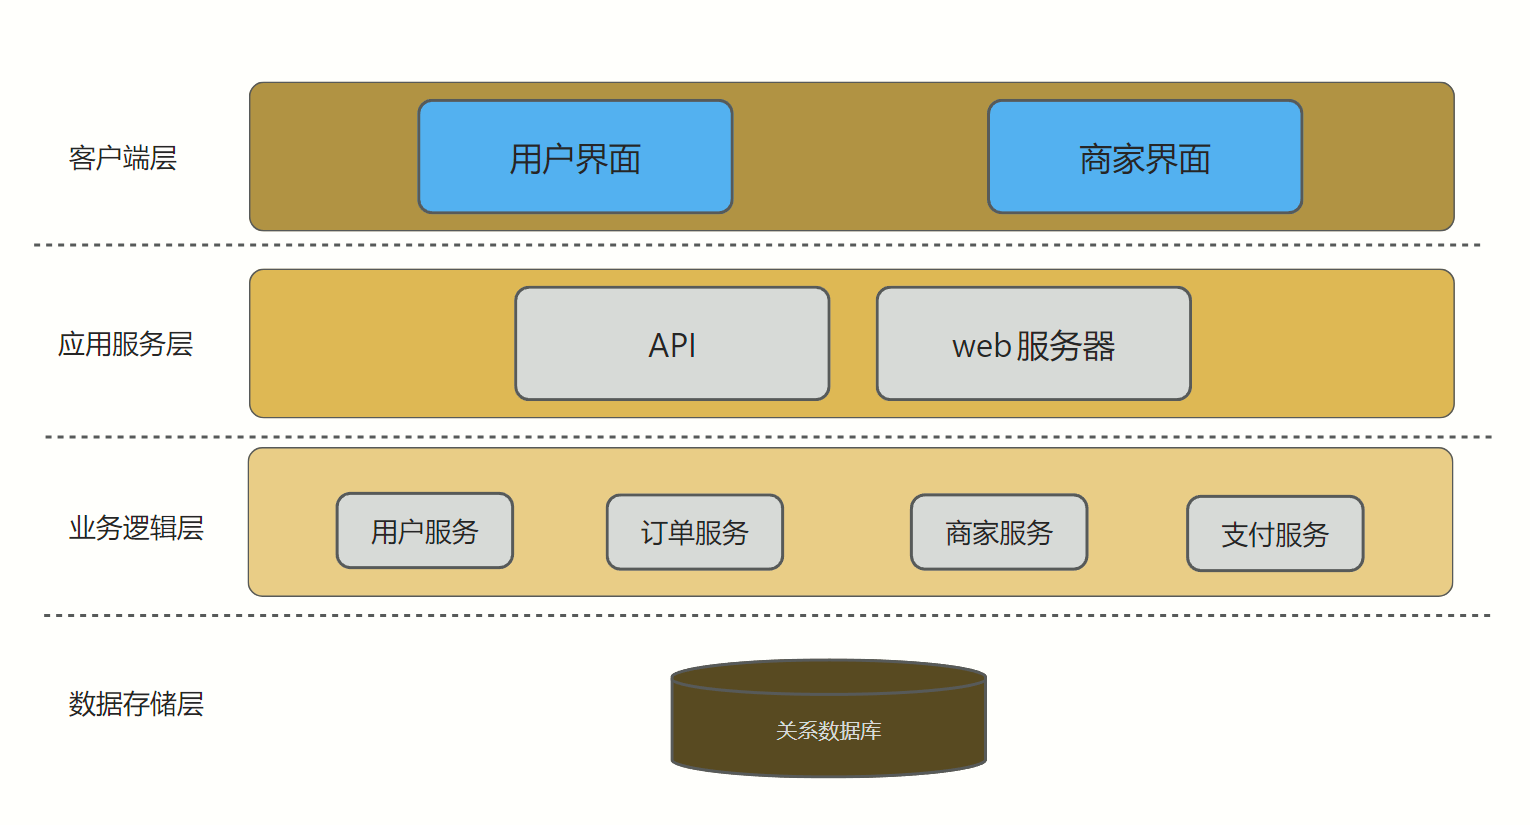
\includegraphics[width=1\linewidth]{pics/14.png}
    \caption{应用架构}
    \label{fig:yyjj}
\end{figure}

\subsubsection{客户端层}
\begin{itemize}
    \item 用户界面:普通用户界面,包含浏览商家、下单、支付、查看订单状态、评价等功能。
    \item 商家界面:商家界面,用于管理订单、商品信息、促销活动等。
\end{itemize}
\subsection{应用服务层}
\begin{itemize}
    \item Web服务器:处理客户端发来的HTTP请求。请求从用户端到Web服务器,然后分发给相应的后端服务。
    \item 负载均衡器:Nginx,用于将请求分发到多个服务实例,确保高并发和高可用性。
\end{itemize}
\subsection{业务逻辑层}
\begin{itemize}
    \item 用户服务:负责用户注册、登录、个人信息管理、地址管理等功能。
    \item 订单服务:负责订单创建、支付、取消、状态跟踪等业务逻辑。
    \item 商家服务:管理商家的信息、商品列表等。
    \item 支付服务(仅模拟实现):集成第三方支付(如支付宝、微信支付),处理支付请求和对账服务。
\end{itemize}
\subsubsection{数据存储层}
\begin{itemize}
    \item 关系型数据库:饿了吧利用MySQL,用于存储结构化数据,如用户信息、订单数据、商家和商品信息。
    \item 缓存系统:如Redis,用于缓存热数据,提升访问速度,减少数据库压力。
\end{itemize}

\subsection{后端 Spring Boot 三层架构}
饿了吧的后端采用Spring Boot三层结构,其应用逻辑分为三个主要层次,分别是 表示层(Controller层)、业务逻辑层(Service层) 和 数据访问层(DAO层)。


\begin{figure}[H]
    \centering
    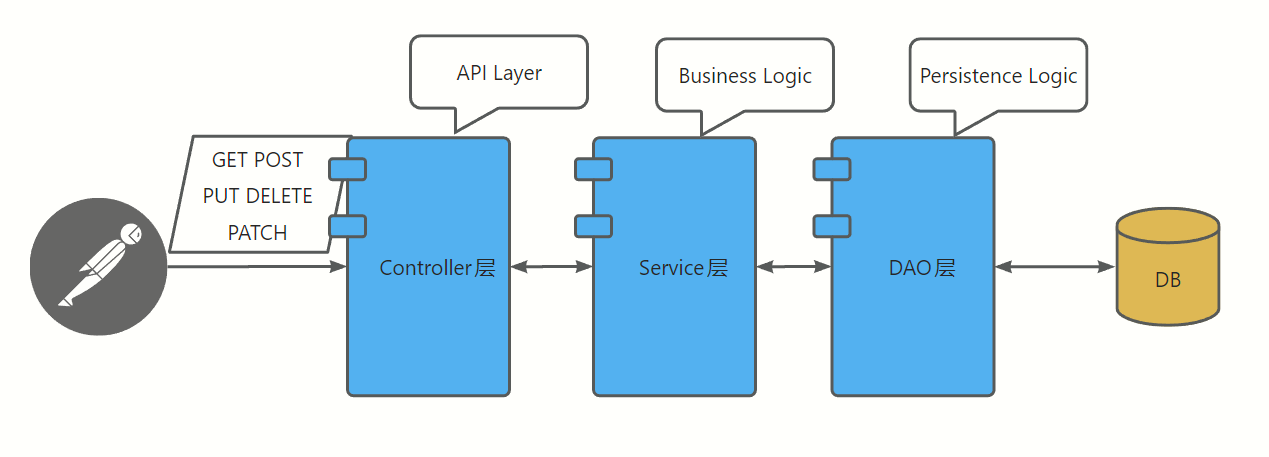
\includegraphics[width=1\linewidth]{pics/15.png}
    \caption{Spring Boot 三层架构}
    \label{fig:scjj}
\end{figure}
表示层负责接收和返回用户请求,业务逻辑层负责核心业务处理,数据访问层则负责与数据库的交互。饿了吧通过这种三层架构,保证代码的高复用性和可测试性。

\section{用户界面设计}
饿了吧的用户界面)和用户体验设计围绕简洁、高效、用户友好等核心原则,旨在为用户提供流畅的点餐、支付、配送跟踪等体验。通过清晰的布局、流畅的导航和实时反馈,饿了吧有效提升了用户点餐、支付、追踪订单的整体体验,符合时代下快节奏的生活方式和需求。
\subsection{首页设计}
\begin{itemize}
    \item \textbf{布局简洁:}饿了吧的首页设计以卡片式布局为主,突出重点信息,如热门商家和推荐菜品.首页的顶部包含一个搜索栏,便于用户快速搜索餐厅。
    \item \textbf{分类导航:}首页常包含美食、超市、生鲜等多种品类的快速导航,帮助用户迅速找到所需的服务.见图\ref{fig:yhjm}。
\end{itemize}
\textbf{UI/UX特点:}
\begin{itemize}
    \item 清晰的导航:首页导航图标简洁、易理解,分类清晰。
    \item 信息优先级明确:通过视觉层次(如字体大小、颜色对比)突出重点信息,如限时优惠、热门餐厅等。
    \item 操作便捷:通过搜索栏,用户可以快速找到想要的餐厅。
\end{itemize}

\subsection{餐厅列表页}
\begin{itemize}
    \item \textbf{餐厅展示}:用户选择某一类目后,会进入餐厅列表页面。每个餐厅的卡片展示餐厅名称、配送费、起送价等核心信息,方便用户比较选择。见图\ref{fig:yhjm}。
\end{itemize}
\textbf{UI/UX特点:}
    \begin{itemize}
        \item 统一的视觉风格:所有餐厅卡片设计风格一致,布局统一,信息一目了然。
    \end{itemize}
 
 
\subsection{餐厅详情页}
\begin{itemize}
    \item \textbf{菜单展示}:点击餐厅进入详情页,用户可以看到详细的菜单分类,菜品按类型排列,并附有图片、价格等信息。
    \item \textbf{购物车浮动按钮}:当用户添加菜品到购物车后,屏幕底部会出现购物车的浮动按钮,实时显示已选商品和价格,方便用户查看和修改订单。见图\ref{fig:yhjm}。
\end{itemize}
\textbf{UI/UX特点:}
\begin{itemize}
    \item 清晰的菜单分类:菜单按照菜品类型分类,用户可以快速找到想要的餐品。
    \item 直观的购物车设计:浮动购物车让用户随时查看订单,避免迷失在复杂的菜品选择中。
\end{itemize}
\begin{figure}[h]
    \centering
    \begin{minipage}[b]{0.3\linewidth}
        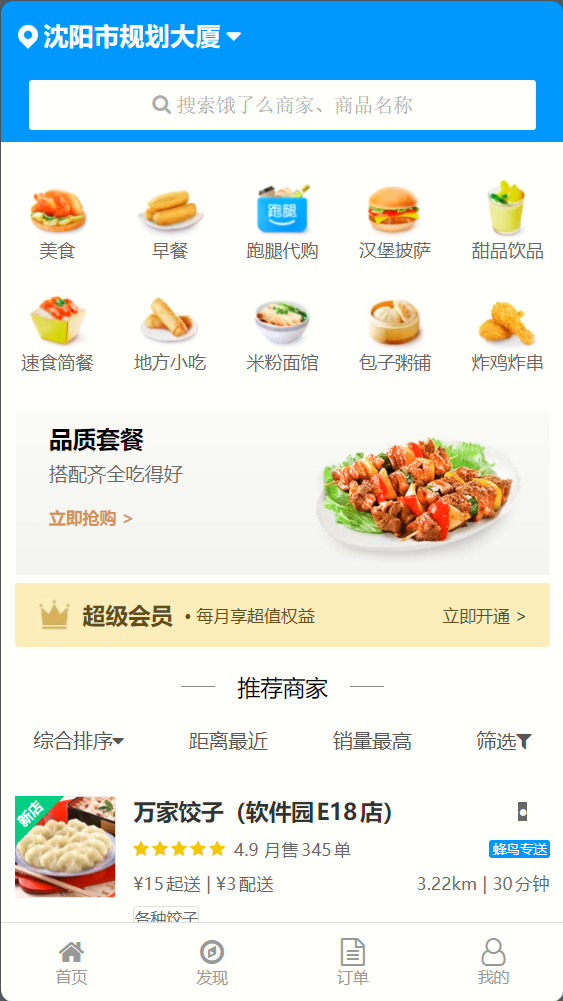
\includegraphics[width=\linewidth]{uiFigs/首页.png}
     \end{minipage}
    % \hspace{0.05\linewidth}  % 调整两图之间的间距
    \begin{minipage}[b]{0.3\linewidth}
        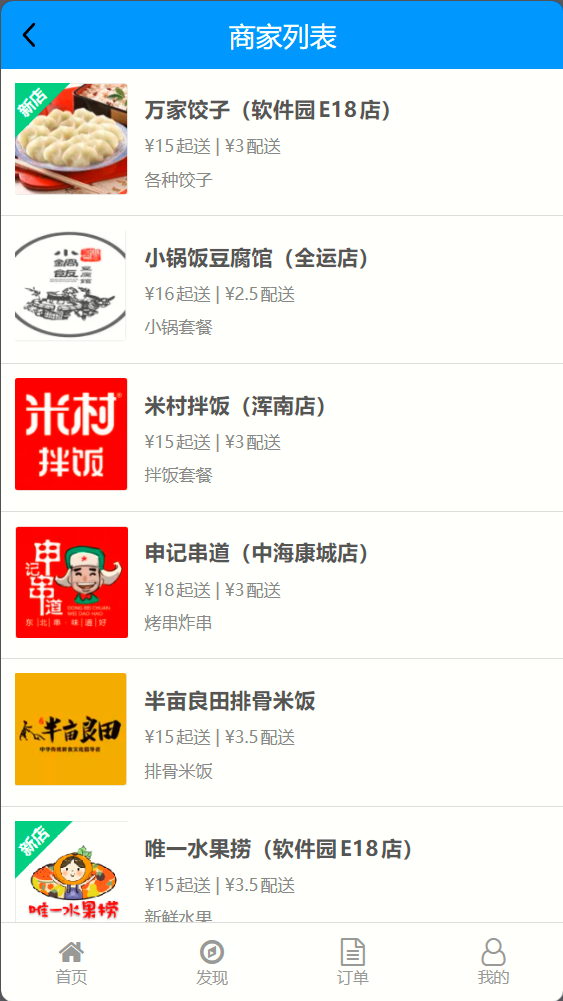
\includegraphics[width=\linewidth]{uiFigs/商家列表.png}
     \end{minipage}
    \begin{minipage}[b]{0.3\linewidth}
        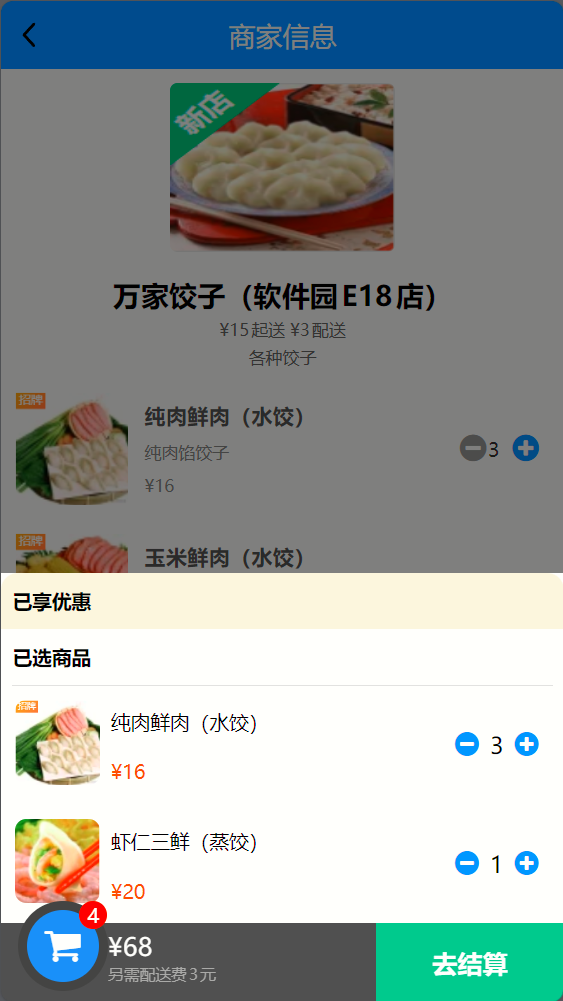
\includegraphics[width=\linewidth]{uiFigs/商家详情.png}
     \end{minipage}
     
    \caption{用户界面}
    \label{fig:yhjm}
\end{figure}

\subsection{订单页}
\begin{itemize}
    \item \textbf{未支付订单}:用户可以清晰的看到当前未支付的订单,并通过去支付跳转到订单支付页面.
    \item \textbf{已支付订单}:用户已支付订单的信息会罗列在这里方便查看.见图\ref{fig:ym2}.
\end{itemize}
 \textbf{UI/UX特点:}
\begin{itemize}
    \item 清晰的订单支付情况概览:用户能够快速了解到订单信息,并对订单进行管理.
\end{itemize}
\subsection{订单确认页}
\begin{itemize}
    \item \textbf{订单概览}:用户在确认订单页可以看到已选菜品、配送费等详细信息,页面设计简洁、条理清晰,帮助用户快速确认订单。
    \item \textbf{地址和支付方式}:用户可以选择配送地址、备注信息和支付方式,并支持多种支付方式,如支付宝、微信支付等。见图\ref{fig:ym2}.
\end{itemize}
 \textbf{UI/UX特点:}
\begin{itemize}
    \item 简化的订单流程:用户可以在同一页面完成订单核对、支付方式选择等多个步骤,减少操作步骤。
\end{itemize}

\subsection{个人中心页}
\begin{itemize}
    \item \textbf{简洁的用户信息展示}:个人中心包括用户头像、用户昵称等信息,用户可以快速查看账户状态。
    \item \textbf{资料管理和地址管理}:用户可以管理配送地址、编辑个人资料等。见图\ref{fig:ym2}.


\end{itemize}
\textbf{ UI/UX特点:}
\begin{itemize}
    \item 模块化设计:信息和功能通过模块化方式展示,减少复杂度。
    \item 易于管理:用户可以轻松找到常用功能,如地址管理等。
\end{itemize}
\begin{figure}[h]
    \centering
    \begin{minipage}[b]{0.3\linewidth}
        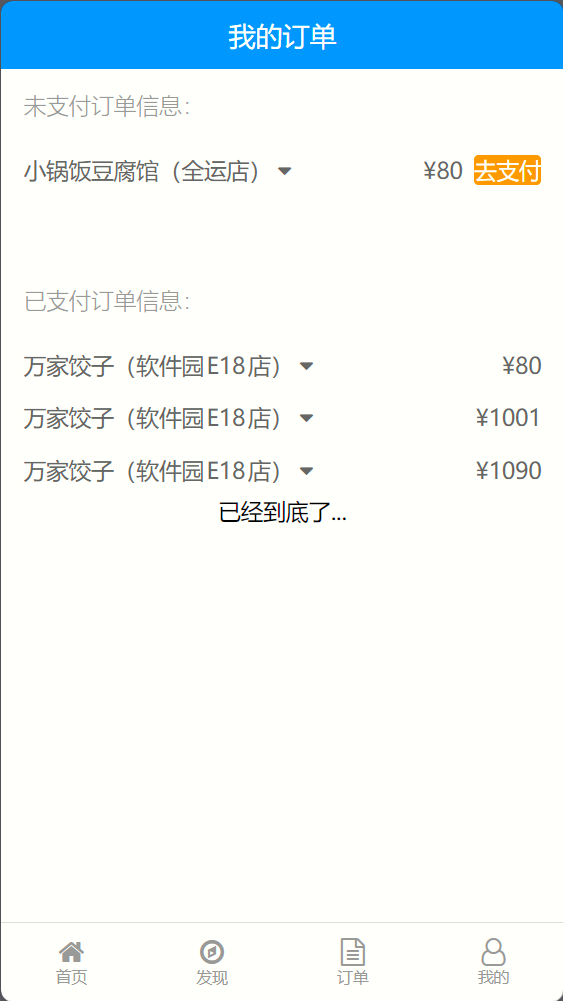
\includegraphics[width=\linewidth]{uiFigs/订单列表.png}
     \end{minipage}
    % \hspace{0.05\linewidth}  % 调整两图之间的间距
    \begin{minipage}[b]{0.3\linewidth}
        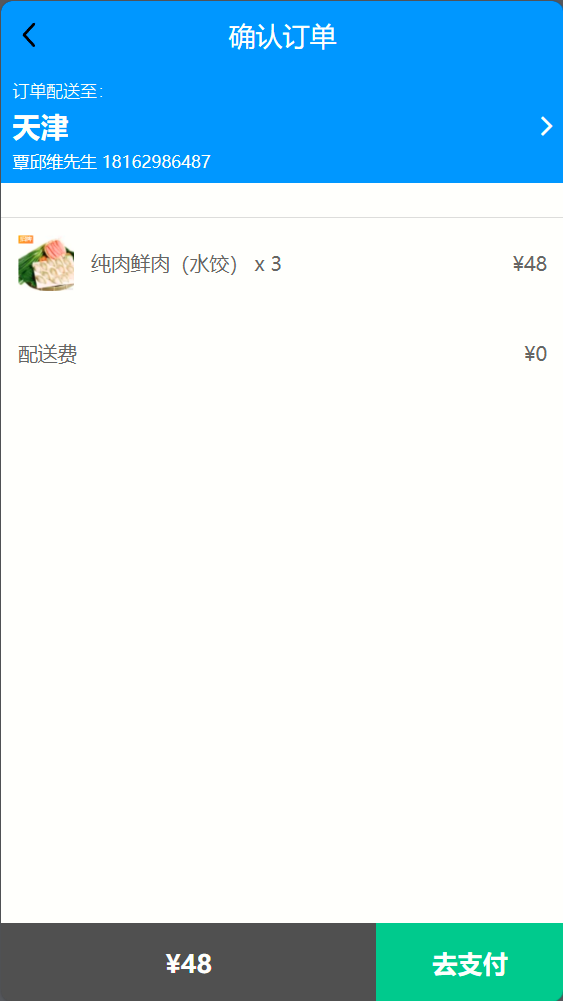
\includegraphics[width=\linewidth]{uiFigs/订单确认.png}
     \end{minipage}
    \begin{minipage}[b]{0.3\linewidth}
        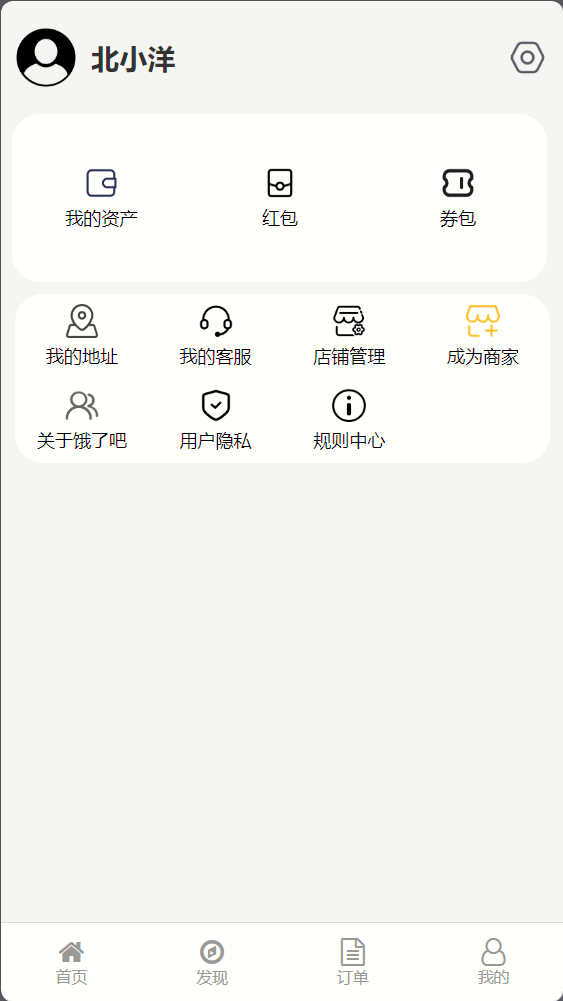
\includegraphics[width=\linewidth]{uiFigs/个人中心.png}
     \end{minipage}
     
    \caption{订单以及个人中心}
    \label{fig:ym2}
\end{figure}



\section{安全设计}
\subsection{密码等隐私数据安全}
后端向前端返回用户信息时,在不需要密码的情景下,后端不会向前端返回密码,而在必须发生前后端密码传输的情景下,饿了吧V2.0将采用如下措施保证密码传输的安全.
\subsubsection{RSA加密}
在前后端分离的系统中,密码的安全性至关重要。饿了吧作为典型的前后端分离式项目,为了在传输过程中保护用户的密码,饿了吧利用 RSA加密算法 在前端对密码进行加密,后端接收到加密后的密码后进行解密。
    
RSA 加密作为非对称加密的典型,加密和解密使用不同的密钥,这种方式可以避免私钥在网络传输中的泄露风险。在饿了吧中,利用Rsa对用户密码进行加密的过程如下:

\begin{enumerate}
    \item 首先OpenSSL生成私钥,并将私钥保存到配置文件中
    \item 后端调用工具类利用私钥生成对应的公钥
    \item 前端申请注册请求时,后端通过public-key接口向前端发送生成的公钥
    \item 前端利用接收到的公钥对明文密码进行加密形成密文,于是在前后端之间传输的内容时密文
    \item 后端接收到前端发来的密文之后通过私钥对密文进行解密得到明文密码
\end{enumerate}
\begin{figure}[h]
    \centering
        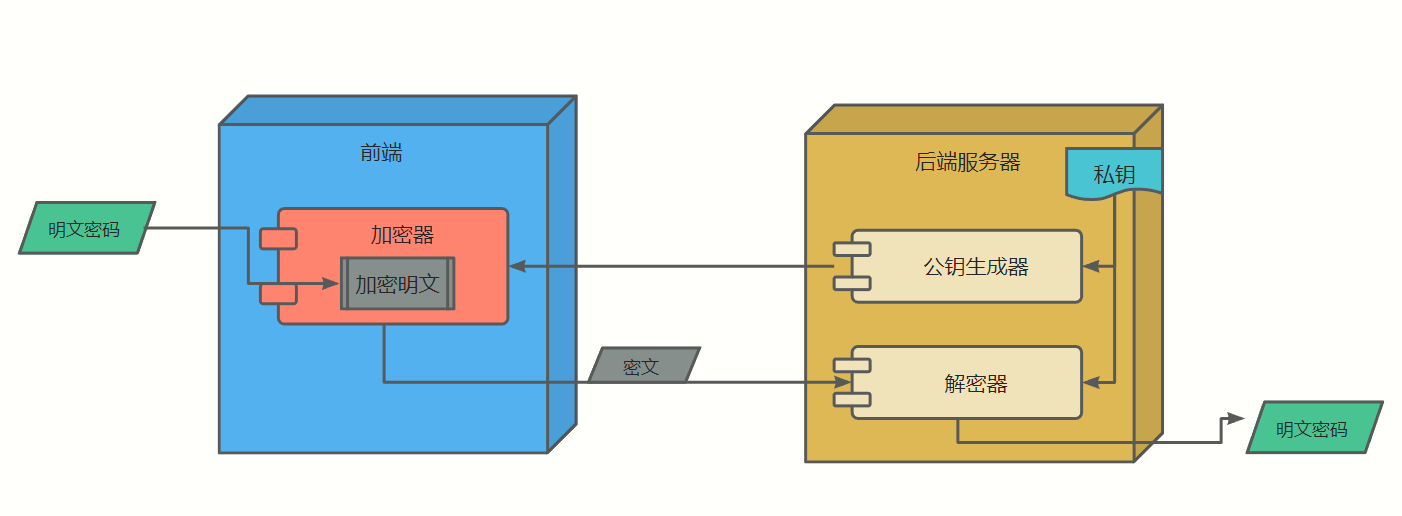
\includegraphics[width=\linewidth]{pics/RSA加密流程.png}
    \caption{RSA密文传输示意图}
    \label{fig:rsa}
\end{figure}
\subsection{加盐加密}
为了预防数据库遭受攻击之后用户的密码信息泄露,提高密码存储的安全性,我们在后端将用户密码存储进数据库时,在原始密码的基础上,添加一个随机生成的值(称为“盐”或 salt),然后再对这个组合进行哈希运算。将得到的哈希值存储进数据库中,其中盐的目的是增加密码的复杂性和唯一性,使得即使用户的密码相同,生成的哈希值也会不同。从而有效保证了密码安全.

\begin{figure}[h]
    \centering
        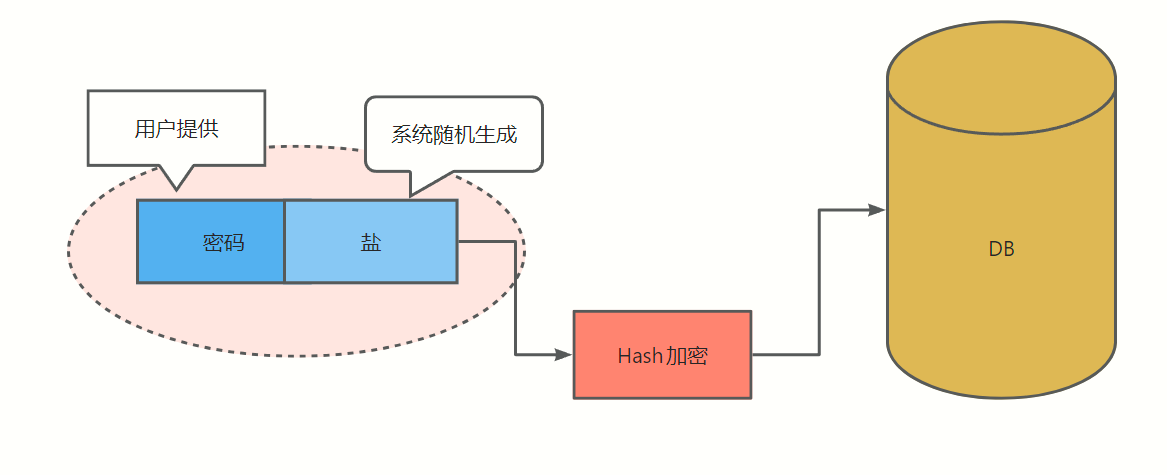
\includegraphics[width=\linewidth]{pics/加盐加密.png}
    \caption{加盐加密示意图}
    \label{fig:jyjm}
\end{figure}

\subsection{身份认证}
饿了吧作为一款前后端分离的系统,为了实现跨域传递的同时实现身份验证机制,饿了吧采用Token(令牌)原理与拦截器共同实现对用户的身份验证,具体实现方法如下:

前端:

在创建好的axios实例axiosInstance上,挂载两个拦截器
\begin{itemize}
\item 请求拦截器:
\begin{itemize}
    \item 前端向后端发送请求之前拦截;
    \item 在header添加token,若有请求错误,在控制台打出
\end{itemize}
\item 响应拦截器:
\begin{itemize}
    \item 后端向前端发送响应,前端接到之后拦截;
    \item 处理响应状态码错误401,500等
    \item 网络错误,重试三次,重试失败,跳转回主页;
    \item 重试次数超过最大限制3,跳转回主页
\end{itemize}
\end{itemize}
后端:

\begin{itemize}
    \item 接到请求后,进入controller层之前拦截;
    \item 登录成功后得到token并发回前端,后所有请求都需加上token;
    \item 被拦截的请求发回500错误码;
    \footnotesize
    \item 注: 拦截涉及用户信息的请求,仅需拦截url的在WebMvcConfig文件配置,需精细到请求方法的在TokenInterceptor配置;
    \normalsize
\end{itemize}

在饿了吧中使用token认证,允许用户在登录后,通过携带 Token 来进行身份认证,而不需要在每次请求时都重新输入用户名和密码。这种方式提高了用户体验,同时保证了系统的安全性。而Token 和拦截器的结合则进一步提供了一种高效、安全、用户体验友好的认证方式。
\begin{figure}[H]
    \centering
    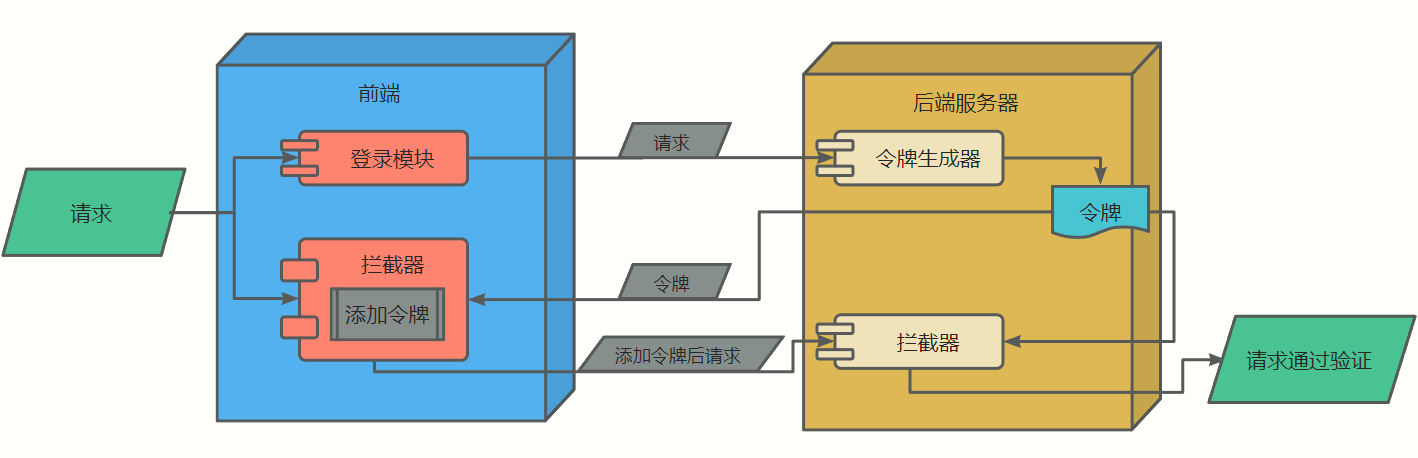
\includegraphics[width=1\linewidth]{pics/token认证.png}
\end{figure}
\subsection{防护策略}\label{con:rjyz}
饿了吧为防止自动化程序或机器人对系统进行恶意操作。提升系统的安全性,使用文字验证码对短时间内进行大量相同请求进行人机验证跳转,在饿了吧业务流程中,主要应用于用户点餐流程中购物车添加过程,当用户往购物车中添加的同一种食品超过一定数量时,系统将提示人机验证,防止机器人或者自动脚本恶意攻击.具体的实现过程如下:

\begin{itemize}
    \item 当前端检测到购物车中同一种商品的数量达到设定值,时,将会请求后端发送文字验证码图片
    \item 文字验证码在后端又系统随机生成,并通过简单的模糊卷积核以及添加噪点的方式对验证码进行模糊化处理并发送到前端
    \item 验证码在前端显示,并提醒用户进行验证
    \item 用户填写的内容发送到后端,后端进行验证,验证通过则前端可以继续操作,否则拒绝前端往购物车中添加食品的请求
\end{itemize}
\begin{figure}[h]
    \centering
    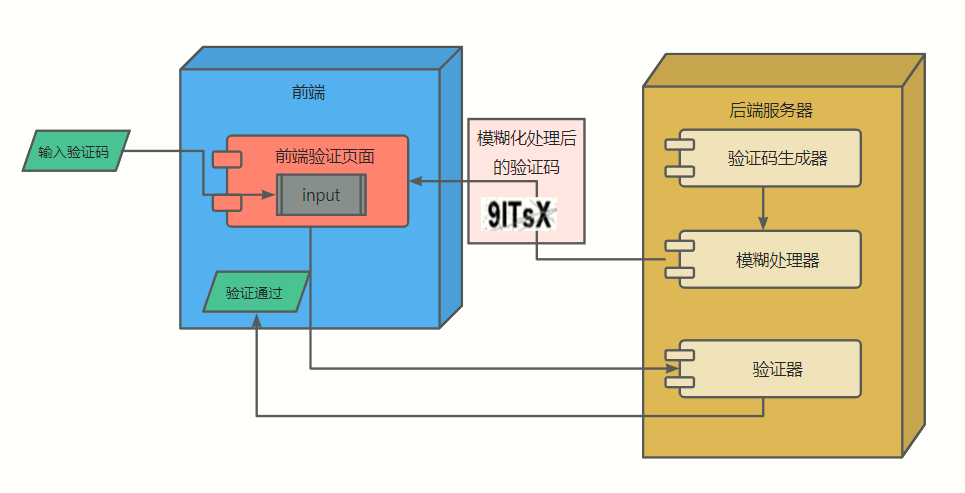
\includegraphics[width=1\linewidth]{pics/人机验证.png}
    \caption{验证码机制示意图}
\end{figure}


\section{细节设计}
\subsection{公用返回组件设计}
考虑到饿了吧1.0中,页面并未添加返回组件,实现页面的返回功能只能依靠浏览器的返回,于是饿了吧2.0中应该设计返回组件作为公用组件,在需要返回功能的页面中导入该组件.

\subsection{显示设计}
饿了吧V1.0中,订单以及购物车的小数显示上存在小数显示的bug, 可以在前端相关位置添加小数显示限定函数进行显示限制.

饿了吧V1.0中,前端版本代码均存在商家列表/食品列表以及首页不能拉到底,最后⼀个信息会被底部菜单栏遮挡的问题,可以通过在底部添加一占位白块解决.

饿了吧V1.0中对于用户的反馈显示使用的是浏览器默认的弹窗提示,用户体验差,饿了吧V2.0将设计专门的提示组件,并对整个项目的前端提示做出重构,提升用户体验.

\subsection{历史订单修改逻辑设计}在对订单中涉及的商品名称、价格以及送货地址等信息进行修改时,会引起历史订单信息的修改.可以通过修改数据库结构,为食品和地址添加删除标记,在删除和修改食品信息或者地址信息时,并非真正的删除和修改,而是将原有数据的删除tag置为1,原数据依旧保留在数据库中,订单读取数据时根据该条数据的唯一id进行查找,依旧是原本的数据.

\subsection{路由添加设计}
饿了吧V1.0中,历史订单的"去支付"并未实现向订单详情的路由,在前端添加相关路由即可实现.

\subsection{手机号验证设计}
在登录/注册以及地址信息的填写中,需要保证手机号格式正确,饿了吧将在前后端进行手机号规范验证,具体内容为:
\begin{itemize}
    \item 手机号不能为空
    \item 手机号位数为11位
    \item 手机号要以1开头
    \item 手机号第二位数字大于2
\end{itemize}
上述验证不仅仅在前端实现,在后端同样需要进行二次验证,并且根据不同的错误返回不同的错误码,正确则由后端返回1,手机号为空返回-1,长度错误返回-2,首位不为1返回-3,格式不正确返回-4.

\subsection{部分逻辑优化设计}
饿了吧V1.0中,后端代码订单业务逻辑缺少对订单和购物车是否为空的验证.在生成购物车时添加对购物车以及订单是否为空的逻辑验证.